% STATUS: ACTIVE -- SSOT for the gain-law SHAPE SELECTION argument (perp axis).
%          Scope ends at "power form rejected, log form adopted".  Wall-generality
%          (curved rigid boundary = cell; slip/permeable = glycocalyx) is NOT here.
% ======================================================
% Compile: xelatex gainlaw_shape_selection.tex
% Path:    reference/eq17_analysis/derivation/gainlaw_shape_selection.tex
% Purpose: Fix the functional form of the motion-gain law BEFORE any filter is
%          built.  Proposal under review (from a slide):
%              a(w-w_s,b,p) = 1 - exp[ -(b/(p+1)) (w-w_s)^(p+1) ],  w_s unknown.
%          Question: may its constants be carried as filter states with
%          [k+1]=[k], i.e. Q = 0?
%
% ---- FORM B ----
%   a = 1 - [ lam / ((w - w_s) + lam) ]^b
%   lam is the LENGTH scale (units of R), not an amplitude, so no fractional
%   power appears.  At w = w_s the bracket is lam/lam = 1 and a = 0 for ANY b:
%   w_s IS the contact position, nominal 1, exactly as Form A and the slide's
%   "w_s - 1: unknown surface position" define it.  One definition of w_s holds
%   for both forms and the fit table reports w_s directly.
%   Far field: 1 - a -> (lam/gap)^b, so at b = 1 lam is the 9/8 reflection
%   coefficient.  b = 1 reduces the form to (w-w_s)/((w-w_s)+lam).
%
%   EQUIVALENT WRITINGS (same family, same fit, same sup; only the label moves):
%     1 - lam_amp*[(w-w_s) + lam_amp^(1/b)]^(-b)   with lam_amp = lam^b
%     1 - lam_amp*(w-w_s)^(-b)                     contact then at w_s+lam_amp^(1/b)
%   The bare last writing is what makes the fitted w_s read -0.063, which is not
%   a surface position; the form above is used precisely so the label matches
%   the meaning.  The amplitude writing needs a fractional power and drags
%   ln(lam)/b^2 terms into every Jacobian; the length writing does not.
%
%   TERM BY TERM AGAINST THE TRUTH (b = 1), cut from the body:
%       bare writing: 1 - lam/w - lam*w_s/w^2 - lam*w_s^2/w^3 - ...
%       truth       : 1 - (9/8)/w +        0/w^2 +    (1/2)/w^3 - ...
%     w^-1 : -lam -> lam = 9/8 ;  w^-2 : -lam*w_s -> w_s = 0 ;  w^-3 unmatched.
%
%   MEASURED (minimax, [1.1,10], 2e4 samples):
%     3 free : lam=1.0566 b=0.9563 w_s=0.9936, sup 0.429%, w_s off by -0.015 um
%              (positioning RMSE is 0.25 um)
%   The table shows each form with its own THREE parameters, so the comparison
%   is like for like: Form A 4.256% against Form B 0.429%, ~10x.
%   Ladder cut from the table: b=1 with lam free gives 0.696%; b=1 and lam=9/8
%   both derived gives 0.779% with w_s the only estimate.
%
%   OPEN, for the estimator not for the form: the 3-parameter Fisher condition
%   number is ~270 on [1.1,10]; cos(lam,b) = 0.979, cos(lam,w_s) = 0.642.
%   Handle it with priors / trajectory design when the filter is built; it is
%   not a reason to change the form.
%
% ---- SCOPE: the PDF is the fit comparison and nothing else ----
%   Cut material, recorded so it is not lost and the cuts are not mistaken for
%   oversights.
%
%   CUT 1 -- the two asymptotic anchors.  Truth: near wall a ~ (w-w_s) exactly
%     (D_perp'(1) = 1); far field 1-a ~ (9/8)/(w-w_s).
%     Form A near wall: a ~ b/(p+1)(w-w_s)^(p+1) = (w-w_s)  =>  p = 0, b = 1.
%     Form A far field: 1-a = exp[...] must decay as a power; for p+1 > 0 it is
%       a stretched exponential, faster than every power  =>  p = -1.
%       => p = 0 and p = -1: no solution, for any (b, w_s).
%     Form A with its own derived b = 1: L k = (w-w_s)^k has NO real root once
%       w > ~2.4 (discriminant -0.20 at w = 2.3, +0.56 at w = 2.5).
%   WHAT THE CUT COSTS: the PDF no longer answers "then add a parameter".  The
%   fit table is a measurement on ONE range with ONE parameterisation; only the
%   anchors make it a ceiling.  Supporting number, also cut: releasing a_o gives
%   Form A four parameters and still only 1.389% (with a_o biased to 0.8915).
%
%   CUT 2 -- wall-position trade-off.  Sweeping the fit's lower bound 1.10 ->
%     2.00 moves Form A's w_s bias +0.113 -> +1.002 um while its sup falls
%     4.256 -> 0.527%: one fixed error budget poured into either pocket.
%     Figure: figures/gainlaw_tradeoff.png.  This is the only evidence bearing
%     on ESTIMATING the surface position, which is why w_s is in the model.
%
%   CUT 3 -- pointwise-solve section and the deficit-tail figure.  Note: with
%     two shape parameters free NEITHER form has constant parameters
%     (A 0.519/0.351).  Figures still produced: gainlaw_constant_A.png, _B.png,
%     gainlaw_deficit_tail.png -- evidence on request, not part of the PDF.
%
% ---- NOTES ----
%  * Every number and figure comes from ONE tracked script:
%        test_script/scratch/gainlaw_shape_evidence.m
%  * Truth = calc_correction_functions (Brenner 1961 series), the same curve the
%    simulator integrates.  No new physics is introduced.
%  * Method: 2e4 log-spaced samples on [1.1,10]; score = sup of the RELATIVE
%    gain error; two-stage (RMS seed -> minimax polish); >= 4 starts; positive
%    parameters carried as logs; w_s guarded below the first sample.  minimax
%    not RMS because the claim is an UPPER BOUND on what a family can do.  The
%    equioscillation count (>= np+1 alternating near-extremal points) rules out
%    "the optimiser did not converge"; all fits reach it.
%  * Range [1.1,10] = operating envelope (config h_init = 20 um -> w = 8.9,
%    h_min = 1.5R with margin below).
%  * lam = 9/8 is the leading Brenner coefficient = Lorentz first reflection,
%    and b = 1 is the Stokes 1/r decay.  Both are derivable, so a fitted
%    lam != 9/8 or b != 1 reads as "this boundary is not a rigid no-slip plane"
%    -- the handle the sequel (curved / slip boundaries) will use.
%
% ---- CONSEQUENCES FOR THE ESTIMATOR (cut from the body 2026-07-30) ----
%   1. Estimate all three (lam, b, w_s); report a_hat only.  The coupling
%      raises the GAIN uncertainty from 0.01% to 0.24% against a 4-5% dominant
%      error elsewhere, so it is not a reason to drop a state.  Dropping to one
%      state costs 1.3% -> 13% on a 7 um cell.
%   2. Do not quote lam_hat or b_hat as physical values and do not put a prior
%      on either alone; corr(ln lam, ln b) = 0.986, only b/lam is determined.
%   3. P carries a 0.99 correlation: use Joseph or UD form for the covariance
%      update, not P = (I-KH)P.  Fisher condition number 355 (three states) is
%      inside double precision (loses ~2.5 of 16 digits) but the loop runs at
%      10 kHz so error accumulates; UD becomes mandatory in single precision.
%   4. Wall geometry, if wanted, comes from a SEPARATE near-wall fit of b/lam
%      over w <~ 1.2.  The operating-range fit underestimates it by 20-30%
%      (e.g. 7 um cell: 1.299 from [1.1,10] vs 1.653 from [1.02,1.2], theory
%      1.746).  Control gain model and wall readout are two different fits.
% ======================================================
\documentclass[11pt,a4paper,fontset=none]{ctexart}
\usepackage[fleqn]{amsmath}
\usepackage{amssymb,bm}
\usepackage{empheq}
\setlength{\mathindent}{0pt}
\usepackage{geometry}
\geometry{margin=2.0cm}
\usepackage{enumitem}
\usepackage{array,booktabs}
\usepackage{titlesec}
\usepackage{graphicx}

\setlength{\parindent}{0pt}
\setlength{\parskip}{0.80em}
\linespread{1.08}
\setlength{\abovedisplayskip}{10pt}
\setlength{\belowdisplayskip}{10pt}
\setlength{\abovedisplayshortskip}{5pt}
\setlength{\belowdisplayshortskip}{5pt}

\newcommand{\wb}{\bar w}
\newcommand{\ws}{\bar w_s}
\newcommand{\ao}{a_{o}}
\newcommand{\g}{(\wb-\ws)}
\newcommand{\hd}[1]{\par\smallskip\noindent\underline{\textbf{#1}}\par\nobreak\vspace{0.1ex}}

\begin{document}

\hd{Normalisation} \;{\small(every length $\div R$; wall plane at $\wb=0$,
contact at $\wb=1$, so $\wb\ge1$)}
\begin{center}\small
\begin{tabular}{@{}ll@{}}
\toprule
$\wb$            & probe-centre position \\
$\ws$            & contact position, unknown; nominal $1$ (surface itself at $\ws-1$) \\
$\g$             & gap between the two surfaces; $0$ at contact \\
$\bar a=a/\ao$   & motion gain, $\in(0,1)$ \\
$b,\;p$          & shape parameters; $\theta=(b,\,p,\,\ws)$ in both forms \\
\bottomrule
\end{tabular}
\end{center}

\hd{Truth} \;{\small(Brenner 1961 series, $\bar a = 1/c_\perp$)}
\[ \bar a(\wb)=1-\tfrac98\wb^{-1}+\tfrac12\wb^{-3}-\tfrac{57}{100}\wb^{-4}
   +\tfrac15\wb^{-5}+\tfrac{7}{200}\wb^{-11}-\tfrac1{25}\wb^{-12} \]

\[ \text{near wall}:\quad \bar a \simeq \g,
   \qquad\qquad
   \text{far field}:\quad 1-\bar a \simeq \frac{9/8}{\g} \]

\hd{Form A} \;{\small(the proposal)}
\begin{empheq}[box=\fbox]{equation*}
 \bar a\g = 1-e^{-\frac{b}{p+1}\g^{\,p+1}}
\end{empheq}

\[ \bar a' = b\,\g^{\,p}\,e^{-\frac{b}{p+1}\g^{\,p+1}} \]

\begin{empheq}[box=\fbox]{align*}
 J_b     &= \bar a'\left[\frac{1}{b}-\frac{\g^{\,p+1}}{p+1}\right] \\[0.5em]
 J_p     &= \bar a'\left[\left(1-\frac{b}{p+1}\g^{\,p+1}\right)\ln\g
            +\frac{b}{(p+1)^2}\g^{\,p+1}\right] \\[0.5em]
 J_{w_s} &= \bar a'\left[b\,\g^{\,p}-\frac{p}{\g}\right]
\end{empheq}

\hd{Two limits of Form A}
{\small near wall, $\bar a\simeq\frac{b}{p+1}\g^{\,p+1}$ must be linear in $\g$:}
\[ p=0,\qquad b=1 \]
{\small far field, $1-\bar a=e^{-\frac{b}{p+1}\g^{\,p+1}}$ must decay as a power;
for $p+1>0$ it decays faster than every power:}
\[ p=-1 \]
\begin{empheq}[box=\fbox]{equation*}
 p=0 \ \wedge\ p=-1 \quad\text{: no solution, for any }(b,\ws)
\end{empheq}

\newpage

\hd{Form B}
\begin{empheq}[box=\fbox]{align*}
 \bar a\big(\wb-\ws,\,b,\,p\big)
   &= 1-\left(1+\frac{\wb-\ws}{b}\right)^{-p}
   &&{\small(\ws-1:\ \text{unknown surface position})} \\[0.45em]
 \bar a\big(\wb-\ws,\,b_w,\,p_w\big)
   &= 1-\left(1+\frac{\wb-\ws}{b_w}\right)^{-p_w} \\[0.45em]
 \bar a\big(\wb_d-\hat{\bar w}_s,\,\hat b_w,\,\hat p_w\big)
   &= 1-\left(1+\frac{\wb_d-\hat{\bar w}_s}{\hat b_w}\right)^{-\hat p_w}
\end{empheq}

{\small equivalently, and the writing used for the derivatives below:}
\[ \bar a\g = 1-\left(1+\frac{\g}{b}\right)^{-p}
            = 1-\left[\frac{b}{\g+b}\right]^{p} \]

\[ \bar a' = p\,b^{\,p}\,\big(\g+b\big)^{-p-1} \]

\begin{empheq}[box=\fbox]{align*}
 J_b     &= \bar a'\left[\frac{p}{b}-\frac{p+1}{\g+b}\right] \\[0.5em]
 J_p     &= \bar a'\left[\frac{1}{p}+\ln\frac{b}{\g+b}\right] \\[0.5em]
 J_{w_s} &= \bar a'\,\frac{p+1}{\g+b}
\end{empheq}

\hd{Two limits of Form B}
{\small near wall, $\g\ll b$, drop the square and higher terms of
$\left(1+\g/b\right)^{-p}\simeq1-p\,\g/b$, then match $\bar a\simeq\g$:}
\[ \bar a \simeq \frac{p}{b}\,\g
   \qquad\Longrightarrow\qquad \frac{p}{b}=1 \]

{\small far field, $\g\gg b$, drop the $1$ against $\g/b$, then match
$1-\bar a\simeq\frac{9/8}{\g}$:}
\[ 1-\bar a \simeq \left(\frac{\g}{b}\right)^{-p} = b^{\,p}\,\g^{-p}
   \qquad\Longrightarrow\qquad p=1,\quad b=\tfrac98 \]

\begin{empheq}[box=\fbox]{equation*}
 \text{over-determined by }12.5\%\ (b=1 \text{ vs } b=\tfrac98),
 \ \text{carried by one parameter}
\end{empheq}

\hd{Under test}
\[ \theta[k+1]=\theta[k], \qquad Q=0 \]

\newpage

\hd{Best-case fit} \;{\small($\wb\in[1.1,10]$, i.e.\ gap $\g\in[0.1,9]$;
minimax, $2\times10^4$ samples)}
\[ \sup\Big|\tfrac{\bar a_{\text{model}}}{\bar a_{\text{true}}}-1\Big| \]

\begin{center}\small
\begin{tabular}{@{}llrrr@{}}
\toprule
form & parameters & $\sup$ [\%] & $\ws-1$ [$\mu$m] & equiosc.\ / starts \\
\midrule
A          & $b{=}0.406,\ p{=}-0.346,\ \ws{=}1.0502$ & $4.256$ & $+0.113$ & 4/4,\; 6/6 \\
\textbf{B} & $b{=}1.0566,\ p{=}0.9563,\ \ws{=}0.9936$ & $\bm{0.429}$ & $\bm{-0.015}$ & 4/4,\; 5/5 \\
\bottomrule
\end{tabular}
\end{center}

{\small Form B against its derived values: $b\,{=}\,1.0566$ vs $9/8=1.125$,
$p\,{=}\,0.9563$ vs $1$.}

\begin{center}
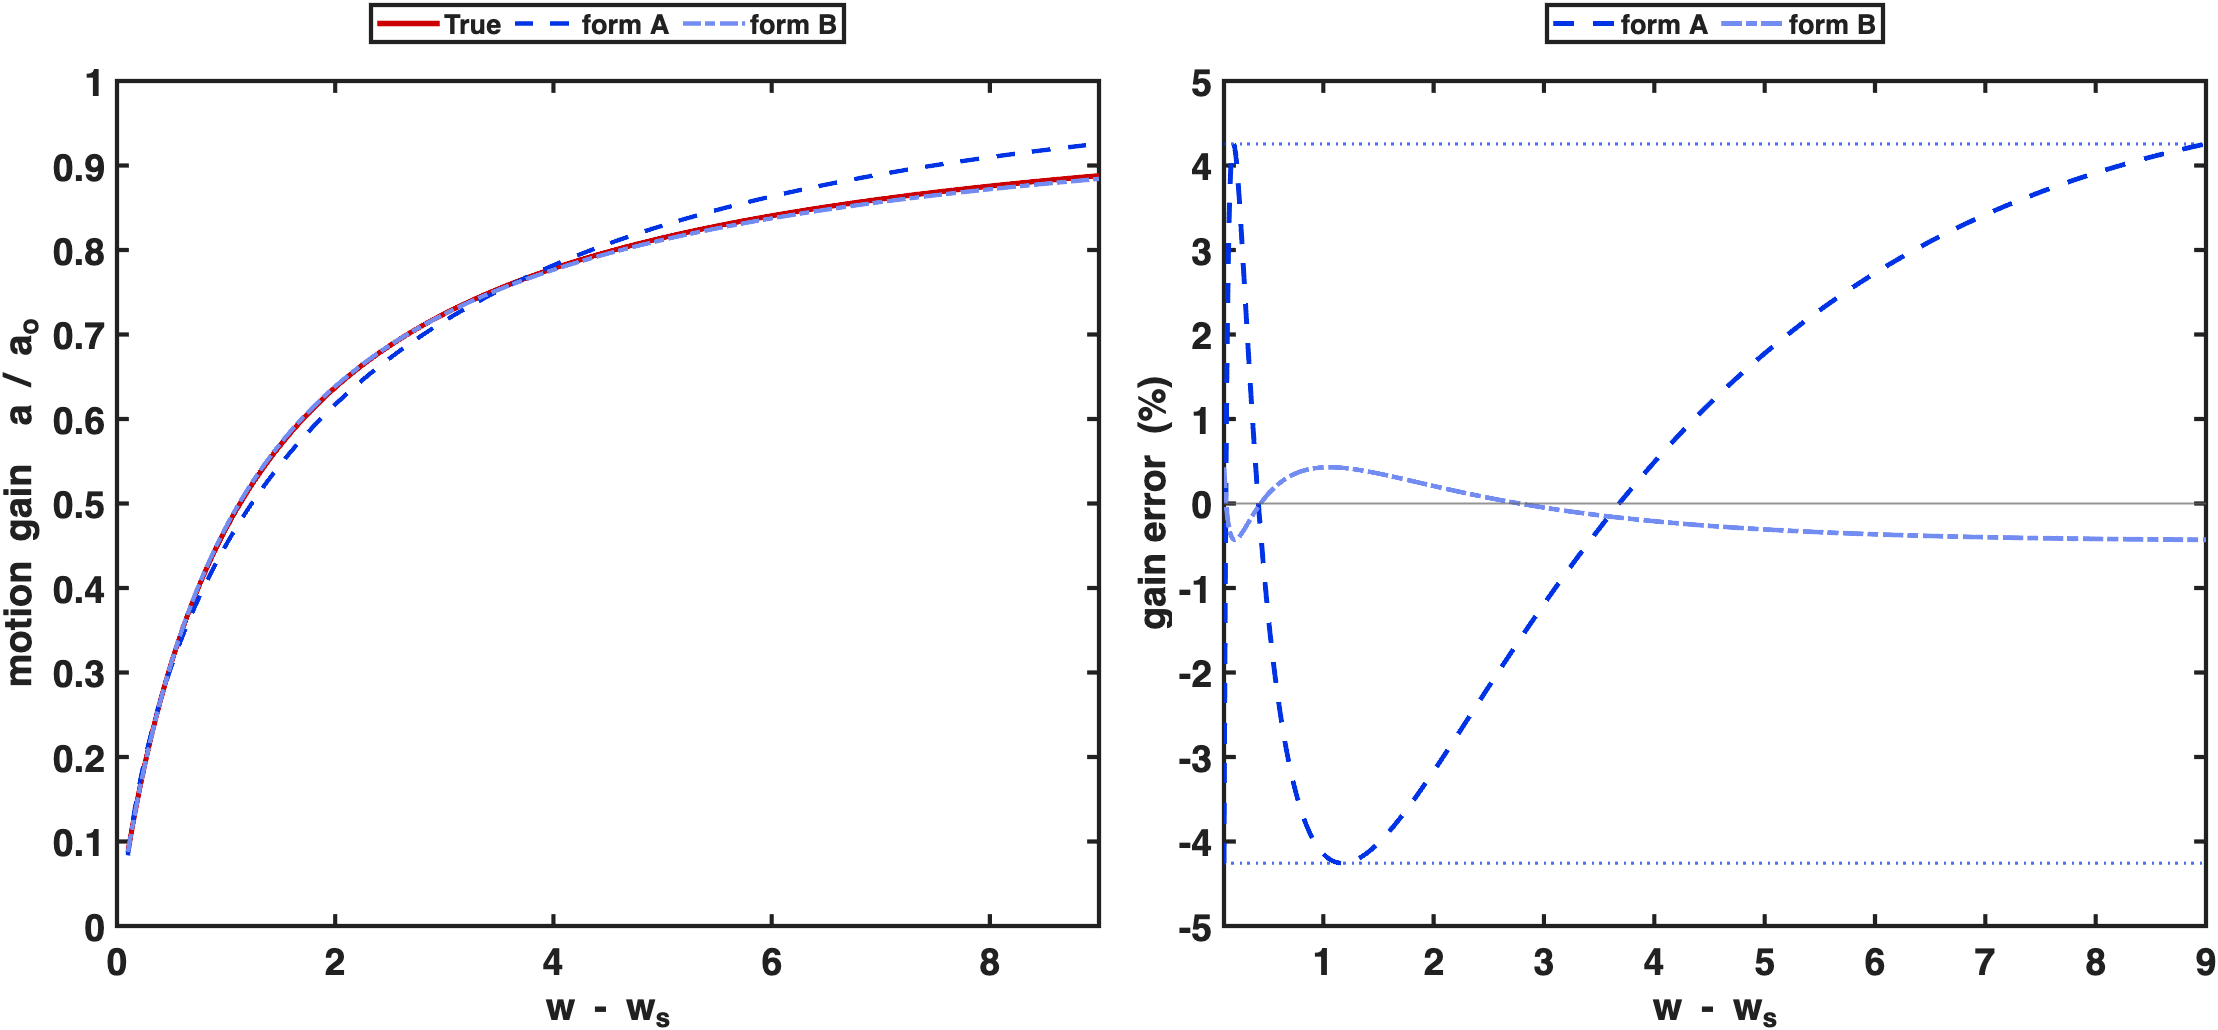
\includegraphics[width=\textwidth]{figures/gainlaw_gain_and_error.png}
\end{center}

\hd{What $b$ and $p$ do} \;{\small(Form B; left $p=1$ with $b$ swept, right
$b=9/8$ with $p$ swept; red is the truth, the middle curve is the derived value)}
\begin{center}
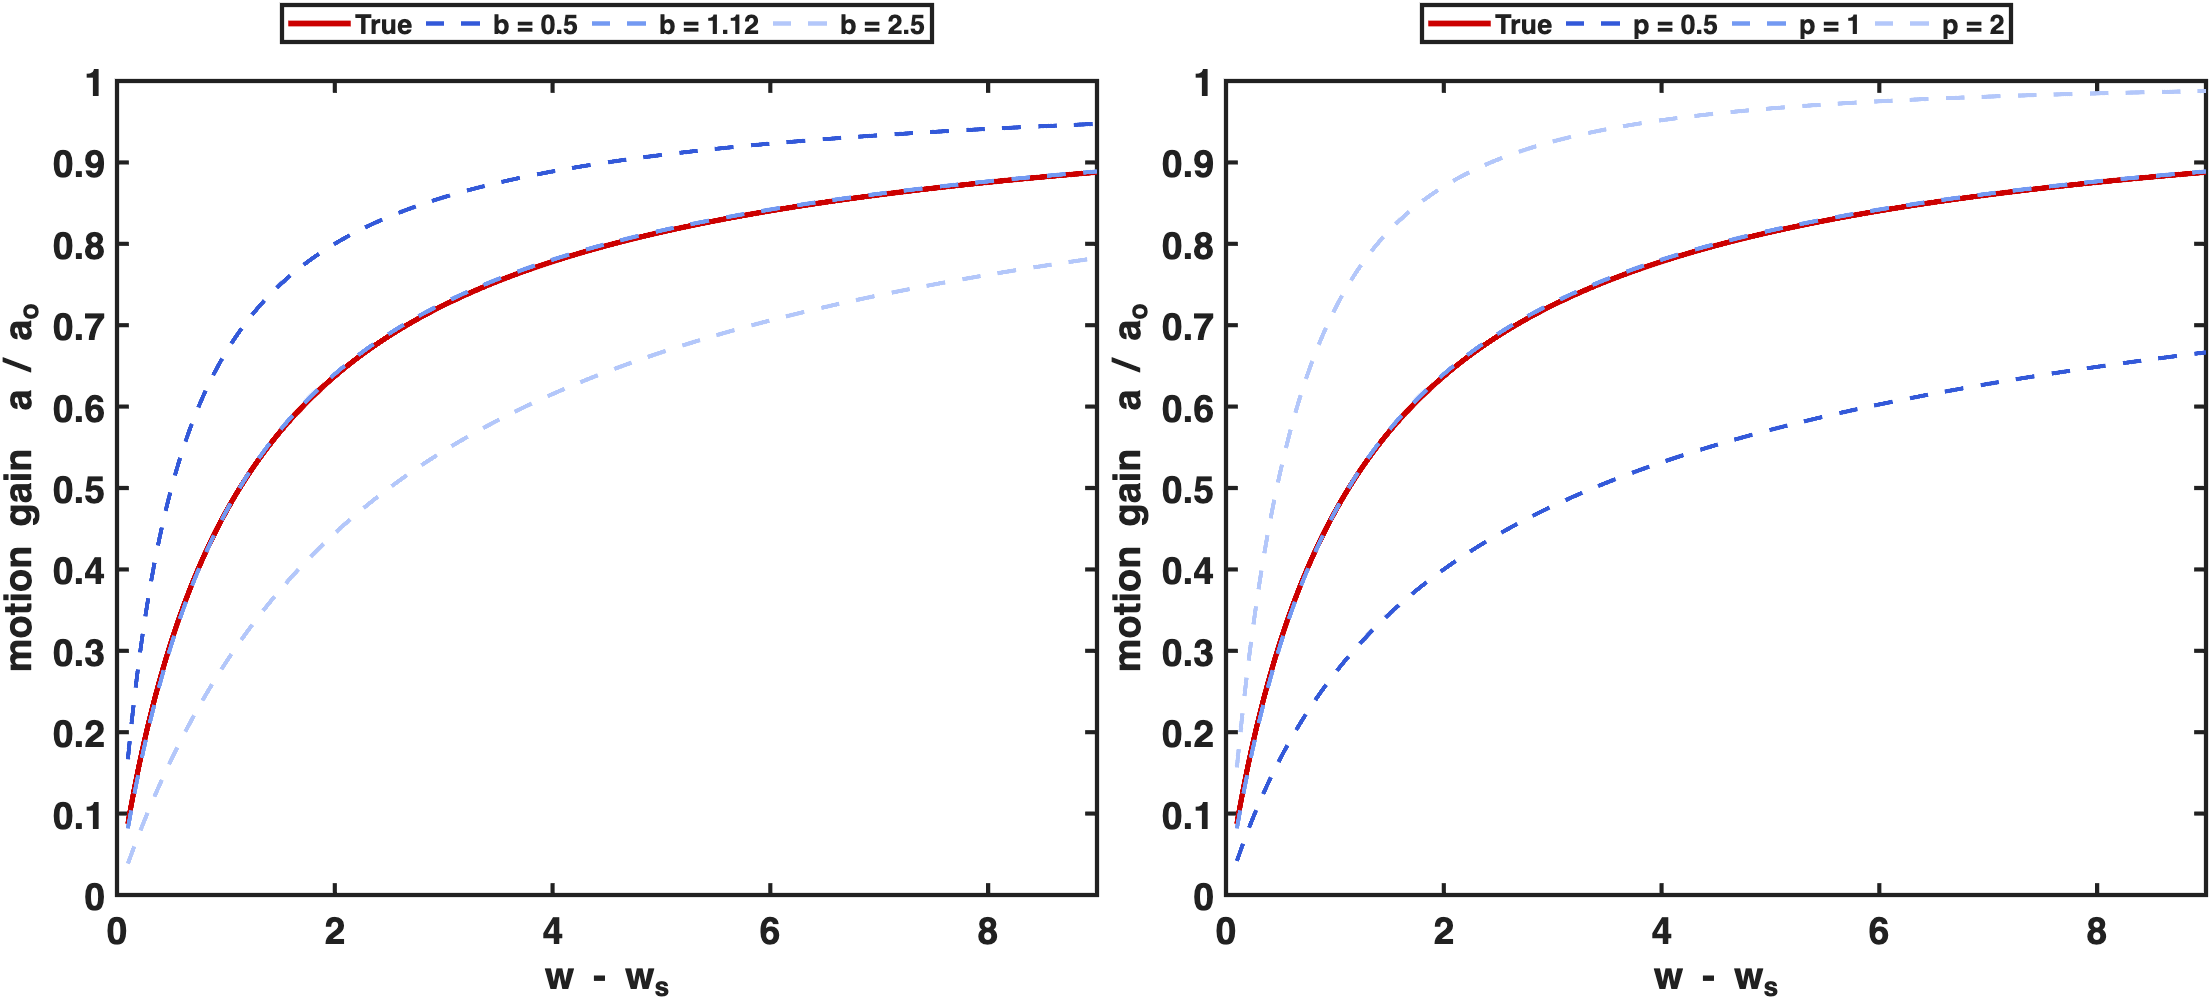
\includegraphics[width=\textwidth]{figures/gainlaw_b_p_roles.png}
\end{center}

\newpage

\hd{The two are not separable} \;{\small(three parameter sets from the floor of
the error valley, each with its own best $\ws$)}
\begin{center}
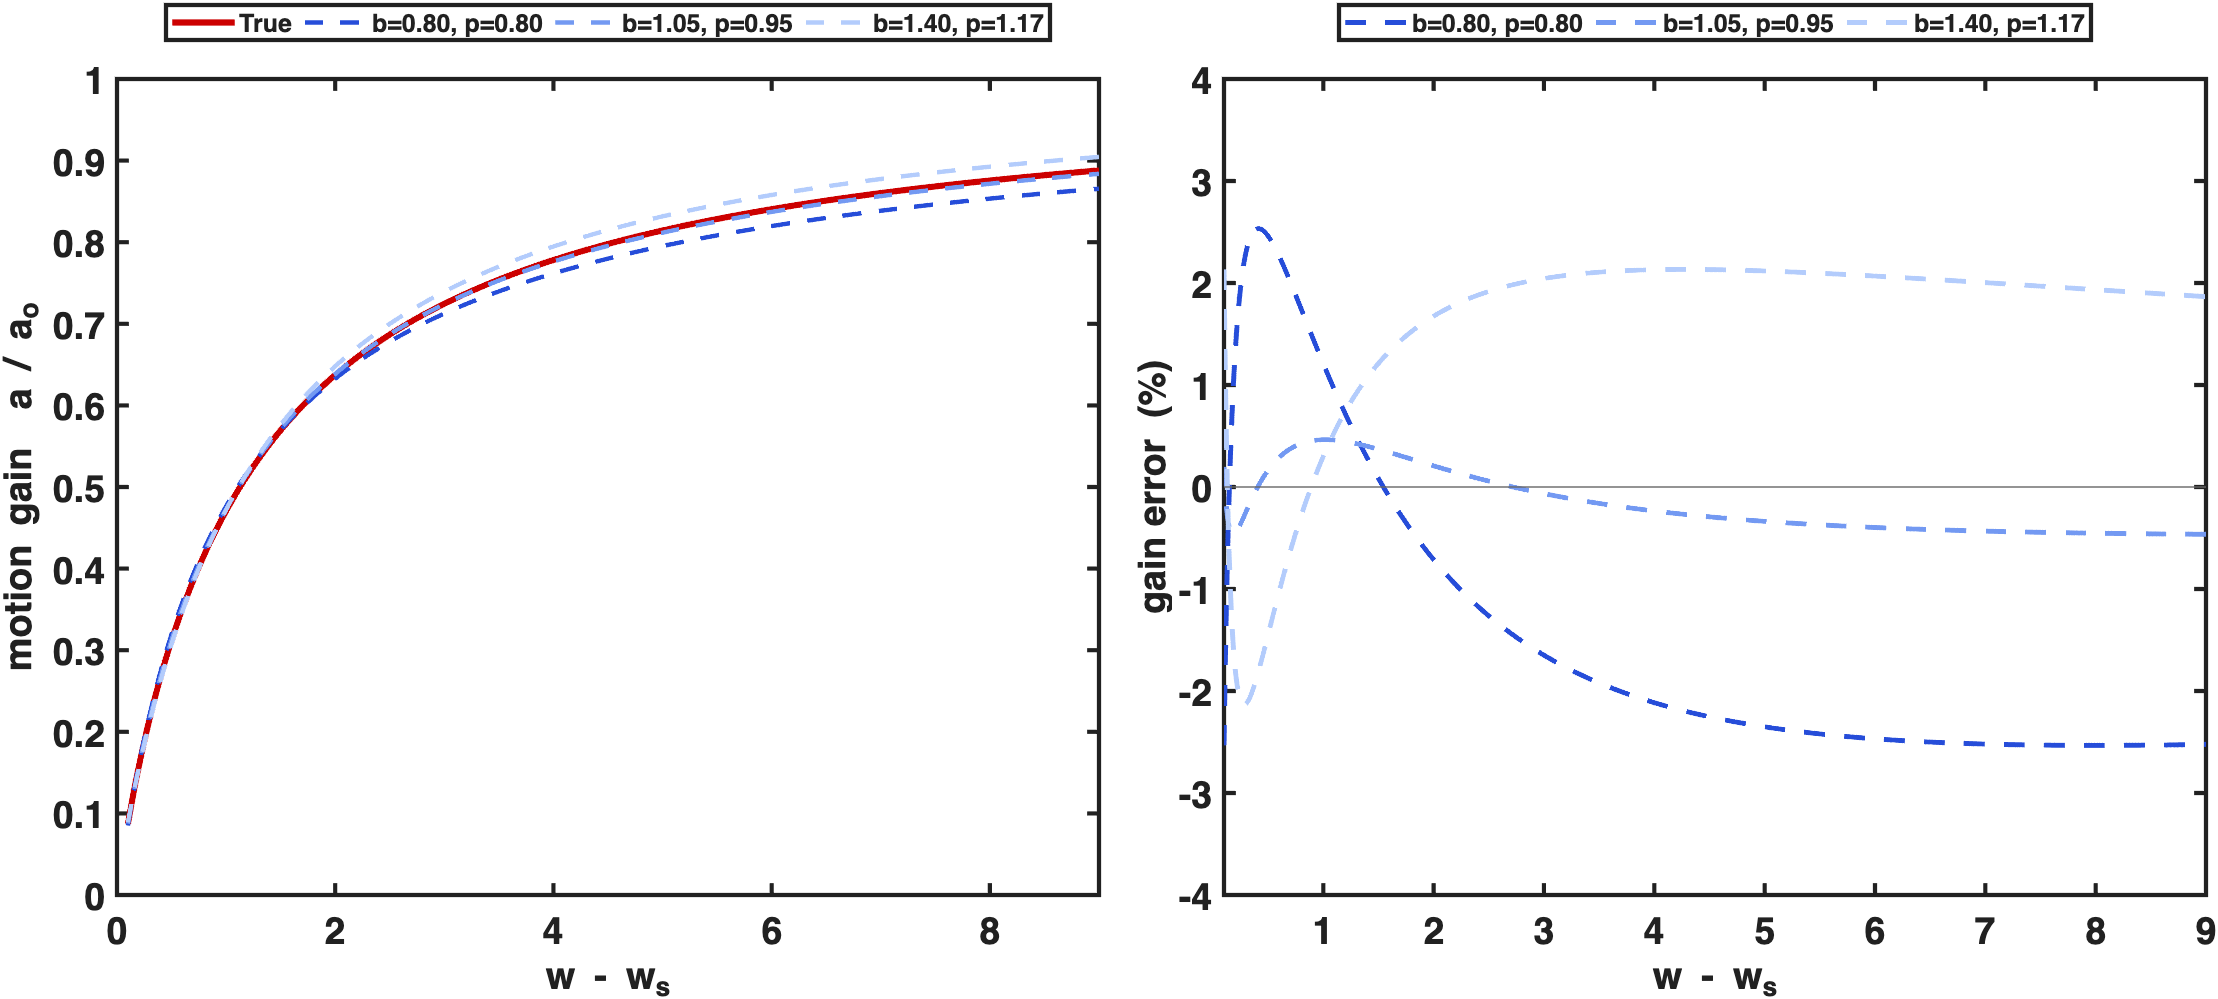
\includegraphics[width=\textwidth]{figures/gainlaw_coupling_demo.png}
\end{center}

\begin{center}\small
\begin{tabular}{@{}rrrrr@{}}
\toprule
$b$ & $p$ & $\ws$ & $p/b$ & $\sup$ [\%] \\
\midrule
$0.80$ & $0.8010$ & $1.0060$ & $1.0013$ & $2.533$ \\
$1.05$ & $0.9528$ & $0.9941$ & $0.9074$ & $0.464$ \\
$1.40$ & $1.1704$ & $0.9837$ & $0.8360$ & $2.133$ \\
\bottomrule
\end{tabular}
\end{center}

\[ b:\ 1.75\times, \qquad p:\ 1.46\times,
   \qquad \text{gain error}:\ <2.6\%,
   \qquad \mathrm{corr}(\ln b,\ln p)=0.986 \]

\end{document}
